\documentclass[12pt]{article}
\usepackage{amsmath}
\usepackage{amssymb}
\usepackage{fancyhdr}
\usepackage{geometry}
\usepackage{hanging}
\usepackage{enumitem}
\usepackage{graphicx}
\usepackage{setspace}
\usepackage{tabularx}
\usepackage{array}
\usepackage{xcolor}
\usepackage{longtable}
\usepackage[table]{xcolor}
%\usepackage{lipsum} %remove later
\doublespacing
%\setlength\parindent{28 pt}
\geometry{letterpaper, margin=1in}

% ++++ Fancy Settings (for header) ++++
\pagestyle{plain}
\fancypagestyle{main}{
	\fancyhf{}
	\lhead{Lab 10}
	\rhead{\leftmark}
	\cfoot{\thepage}
	\renewcommand{\headrulewidth}{0.4pt}
}

% Column widths (tweak the numbers if you want)
\newcommand{\colNum}{0.06\linewidth}   % column 1 (1–10)
\newcommand{\colSmall}{0.16\linewidth} % columns 2,3,5
\newcommand{\colBig}{0.48\linewidth}   % column 4 (3x colSmall)

% ++++ Begin Doc ++++

\begin{document}

% ++++ Cover Page ++++

\begin{titlepage}
\centering
\vfill

% ++Logo

\includegraphics[width=0.35\textwidth]{images/logo.png}

\vspace{1.5cm}

% ++Title
\LARGE{\textbf{Lab 10: Vulnerability Scanning}}\\
\vspace{0.3cm}
\large{\textbf{Keith Schoen}}\\
\vspace{0.3cm}
\large{\textbf{CSEC3755-001}}\\
\vspace{0.3cm}
\large{\textbf{Dr. Daniel Pittman}}\\
\vspace{0.3cm}
\large{\textbf{16 April 2026}}\\
\vspace{0.3cm}

\vfill
\end{titlepage}

% ++++ ToC ++++

\pagenumbering{gobble} %hide page numbers for cover and ToC
\tableofcontents
\clearpage

% ++++ Begin Report ++++

\pagenumbering{arabic} %page one starts here
\setcounter{page}{1}
\pagestyle{main} %turn on fancy

% ++++ Part 01 ++++
\section{Network Discovery with Nmap}

% +++ 1.1 +++
\subsection{Host Discovery Scan}
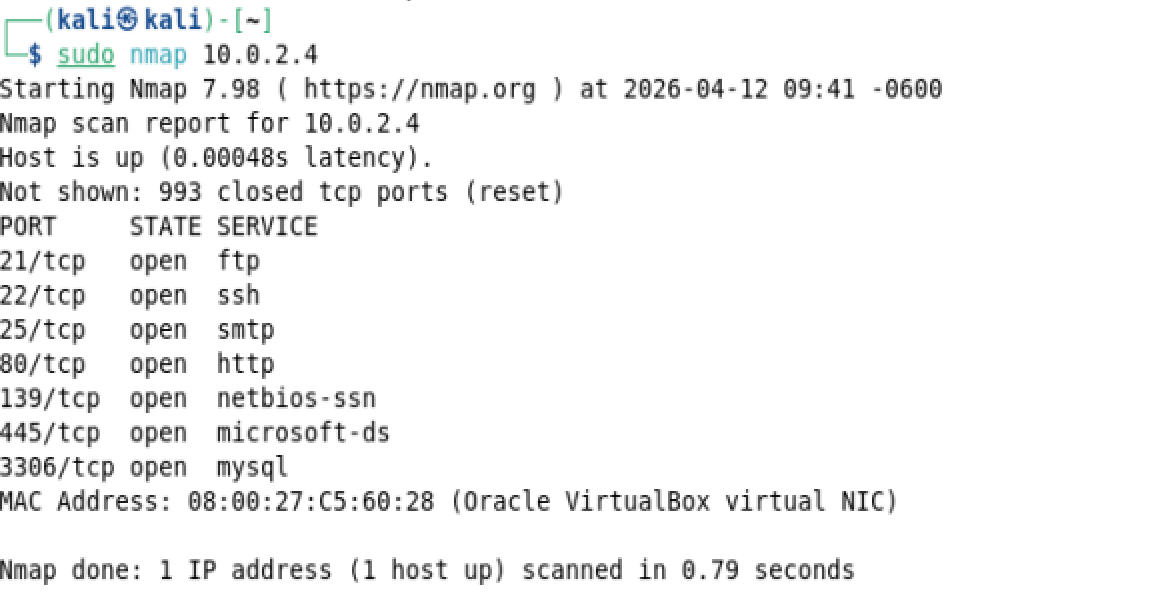
\includegraphics[width=0.8\textwidth]{images/1.1.png}\\ \textit{Figure 1: Nmap host discovery scan results.}

% +++ 1.2 +++
\subsection{Service Version Detection}
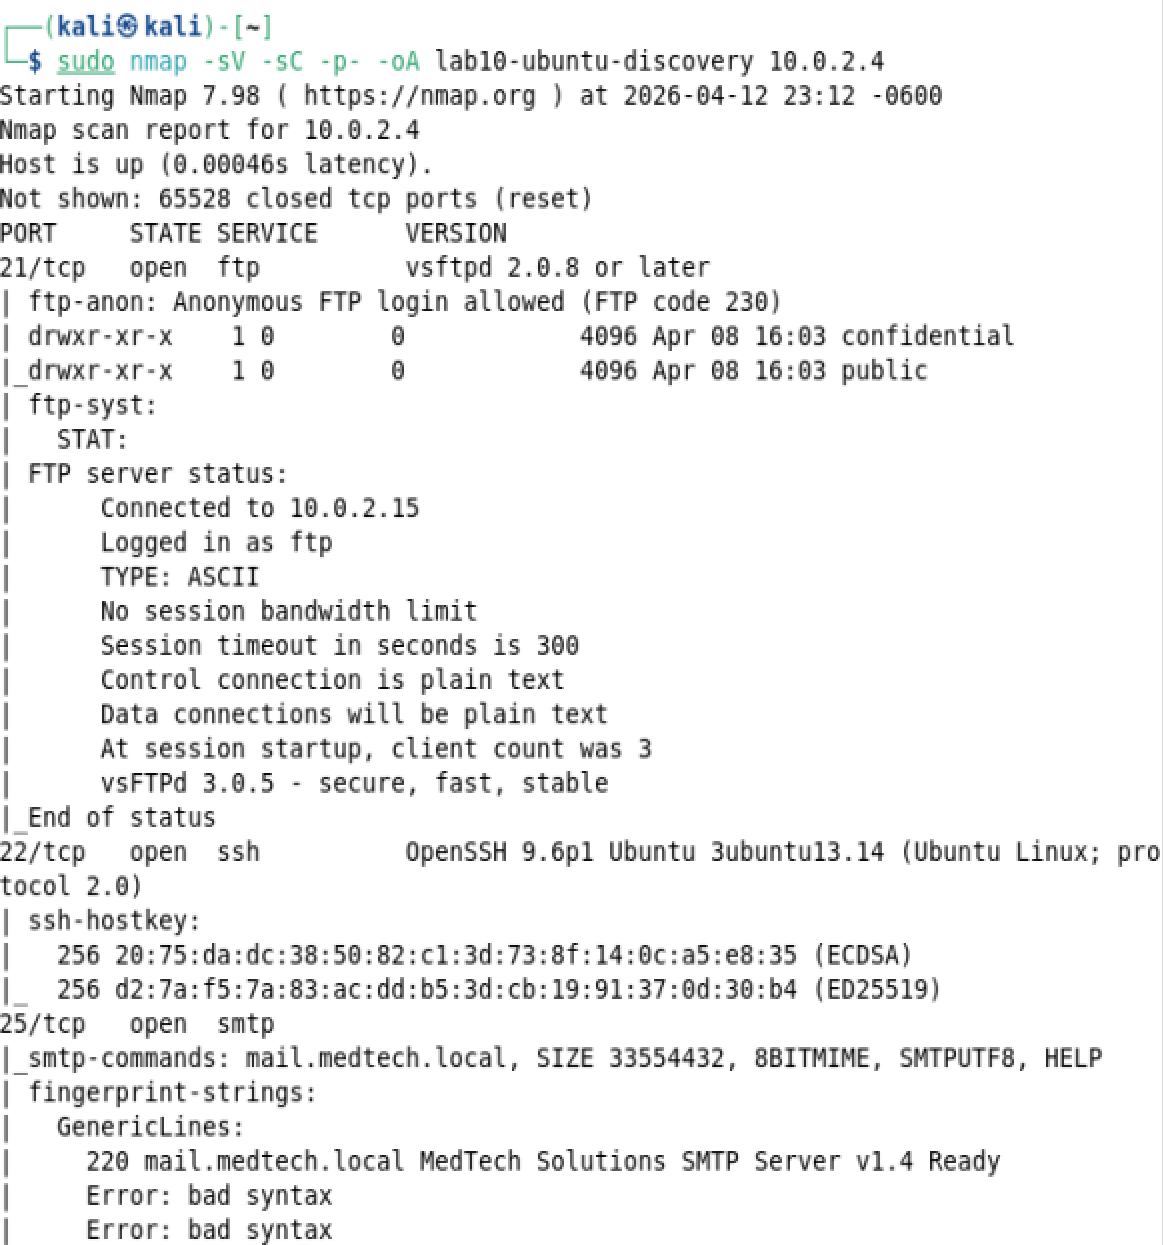
\includegraphics[width=0.60\textwidth]{images/1.2.1.png}\\ 
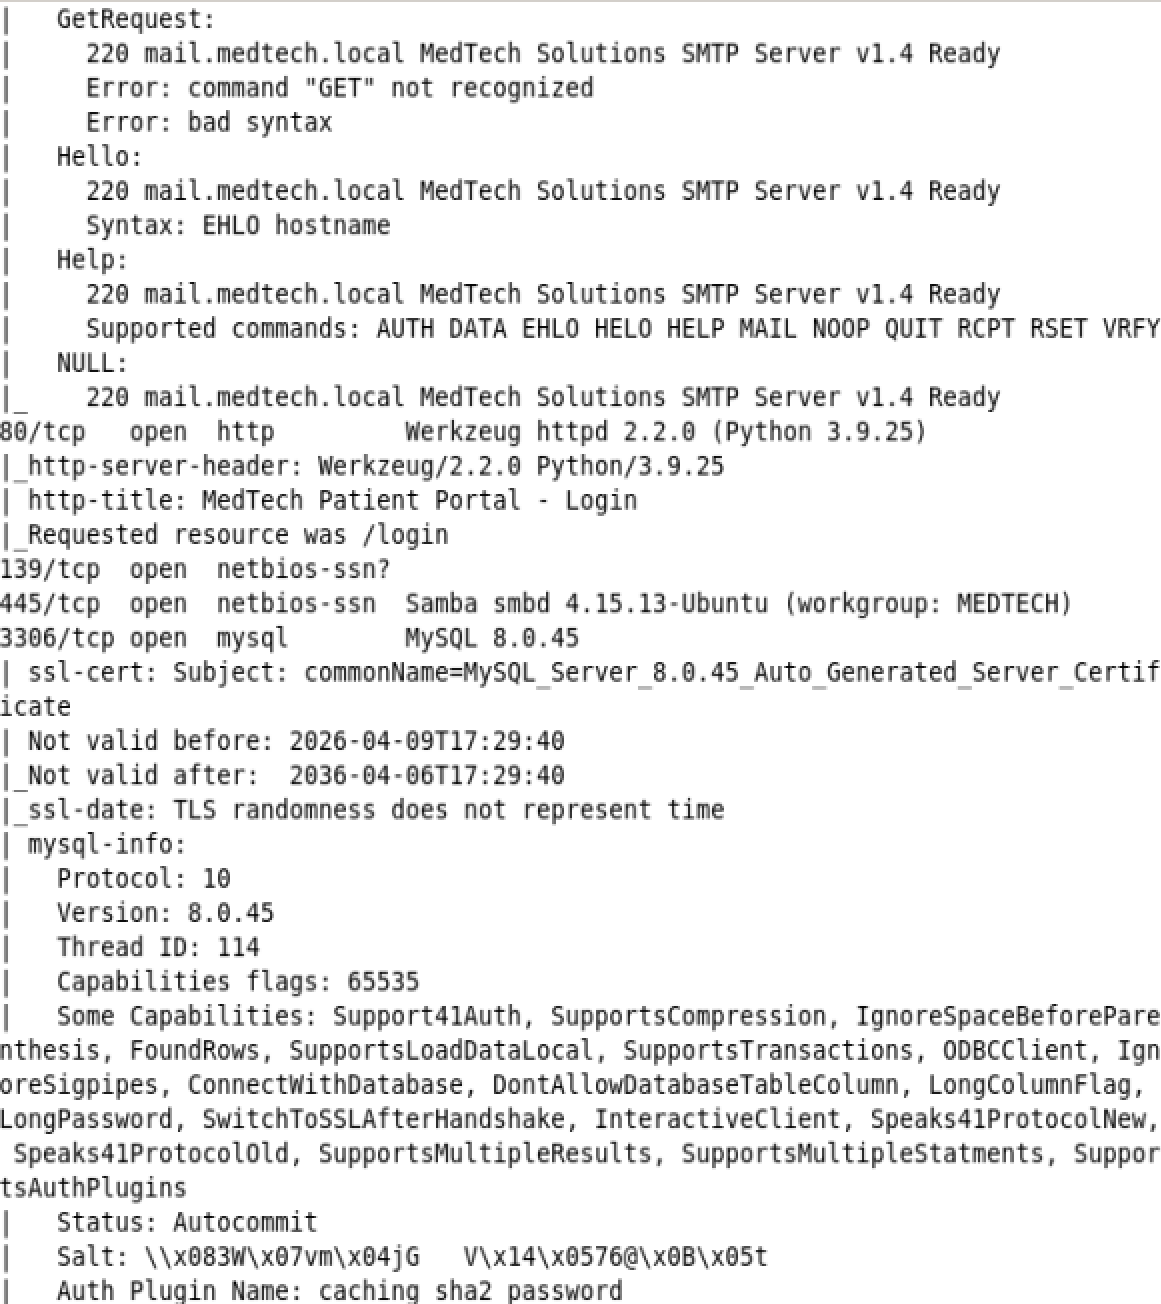
\includegraphics[width=0.60\textwidth]{images/1.2.2.png}\newpage 
\noindent 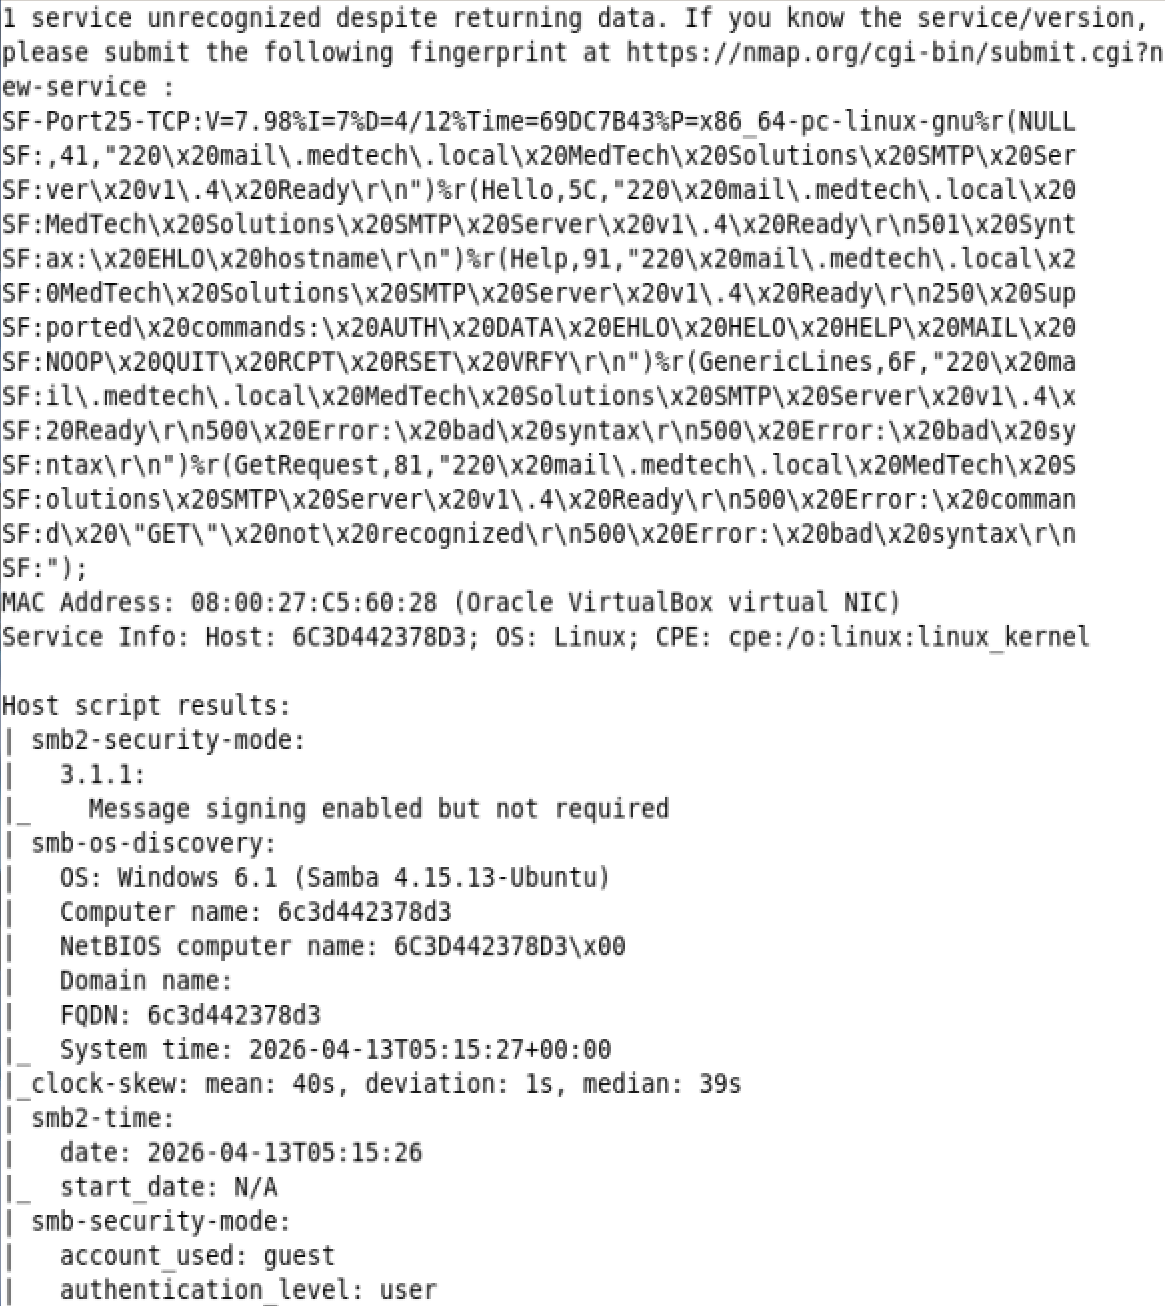
\includegraphics[width=0.60\textwidth]{images/1.2.3.png}\\ 
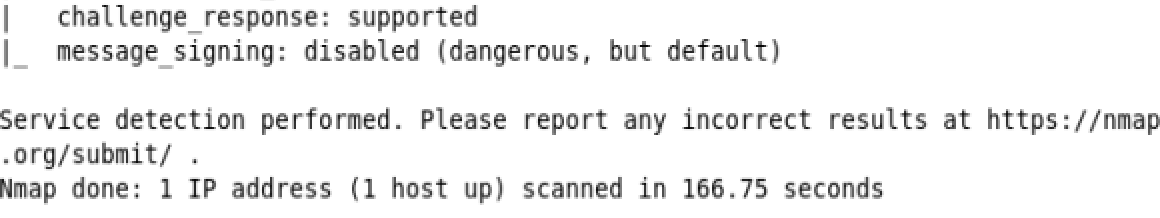
\includegraphics[width=0.60\textwidth]{images/1.2.4.png}\\ 
\textit{Figure 2: Nmap service version detection results.}

% +++ 1.3 +++
\subsection{OS Detection}
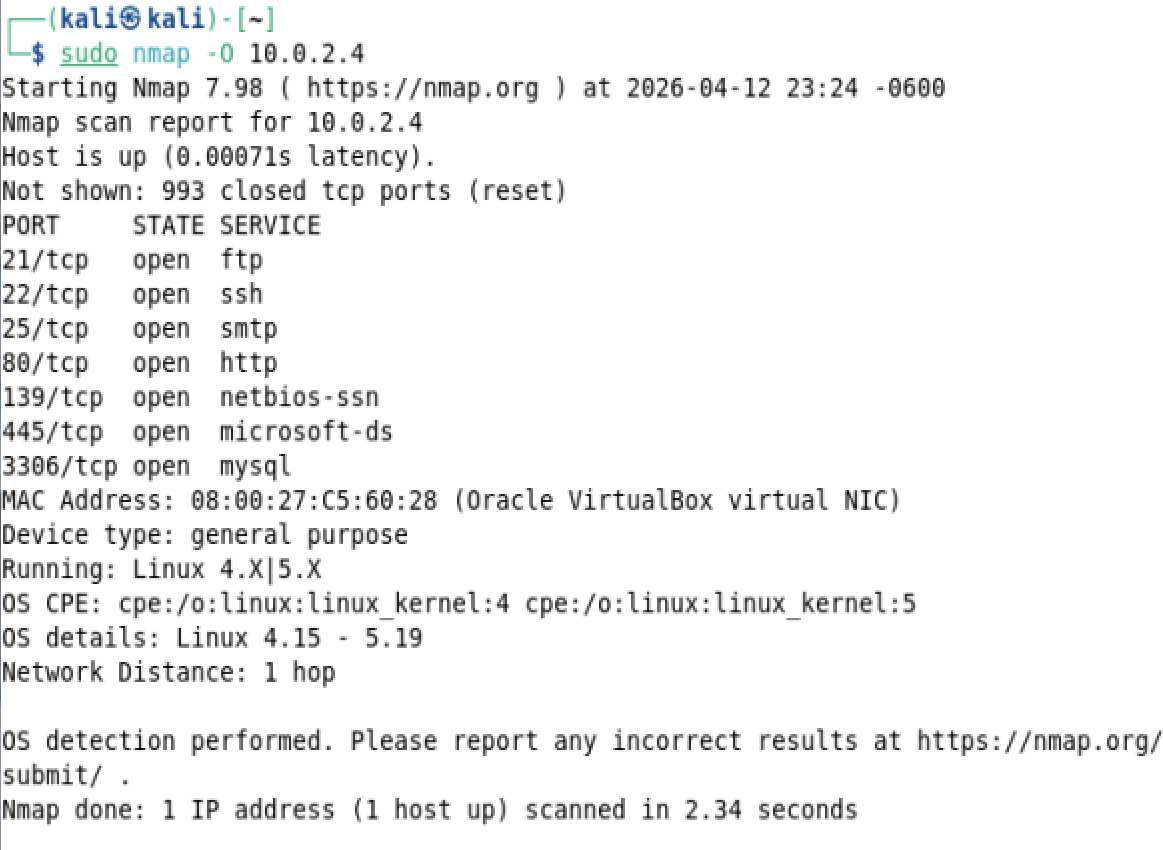
\includegraphics[width=0.8\textwidth]{images/1.3.png}\\ \textit{Figure 3: Nmap OS detection results.}
\newpage
\subsection {Documentation}

{\singlespace
    \begin{longtable}{
        || >{\centering\arraybackslash}p{\colNum}
        | >{\raggedright\arraybackslash}p{\colSmall}
        | >{\raggedright\arraybackslash}p{\colBig}
        | >{\raggedright\arraybackslash}p{\colSmall} ||}
        \hline
        \textbf{\small Port \& Protocol} &
        \textbf{\small Service Name \& Version} &
        \textbf{\small What this service does} &
        \textbf{\small Should it be externally accessible and why} \\
        \hline\hline
        \endfirsthead
        \hline
        \textbf{\small Port \& Protocol} &
        \textbf{\small Service Name \& Version} &
        \textbf{\small What this service does} &
        \textbf{\small Should it be externally accessible and why} \\
        \hline\hline
        \endhead
        \hline
        \endfoot
        \hline\hline
        \endlastfoot
        21 TCP & FTP (vsftpd 2.0.8+) & File Transfer Protocol, used for transferring files between hosts; this instance allows anonymous login with no encryption. & No. Unencrypted and anonymous access is a serious risk; use SFTP instead. \\
        \hline
        22 TCP & SSH (OpenSSH 9.6p1) & Secure Shell, used for secure remote login and command execution. & Limited. Restrict to known IPs or a VPN; never expose to the open internet. \\
        \hline
        25 TCP & SMTP (MedTech SMTP v1.4) & Simple Mail Transfer Protocol, used for sending emails between servers. & No. Open SMTP relays invite spam abuse; the VRFY command is also exposed, creating a user enumeration risk. \\
        \hline
        80 TCP & HTTP (Werkzeug 2.2.0/Python 3.9.25) & Hypertext Transfer Protocol, used for serving web pages. & No. A patient portal must use HTTPS (port 443); plain HTTP transmits credentials and PHI in cleartext. \\
        \hline
        139 TCP & NetBIOS-SSN (Samba, legacy) & Legacy Windows networking protocol used for file and printer sharing on local networks. & No. NetBIOS should never be internet-facing; it is a common target for lateral movement attacks. \\
        \hline
        445 TCP & SMB (Samba 4.15.13-Ubuntu) & Windows file-sharing protocol that allows shared drives and printers across a network. & No. SMB exposed externally is extremely dangerous (WannaCry, EternalBlue); message signing is also disabled on this host. \\
        \hline
        3306 TCP & MySQL (MySQL 8.0.45) & Relational database management system storing application data. & No. Databases should never be directly internet-facing; access should only occur via the application layer on localhost. \\
        \hline
    \end{longtable}
}
\noindent \textit{Table 1: Documentation of discovered services. \\ After logging my inital findings, I rand the results through Claude to see what else it found. The final three entries (and the note about VRFY in port 25) are results of its findings.}

% ++++ Part 02 ++++
\section{Nmap Vulnerability Scanning (NSE)}

% +++ 2.1 +++
\subsection{General Vulnerability Scan}
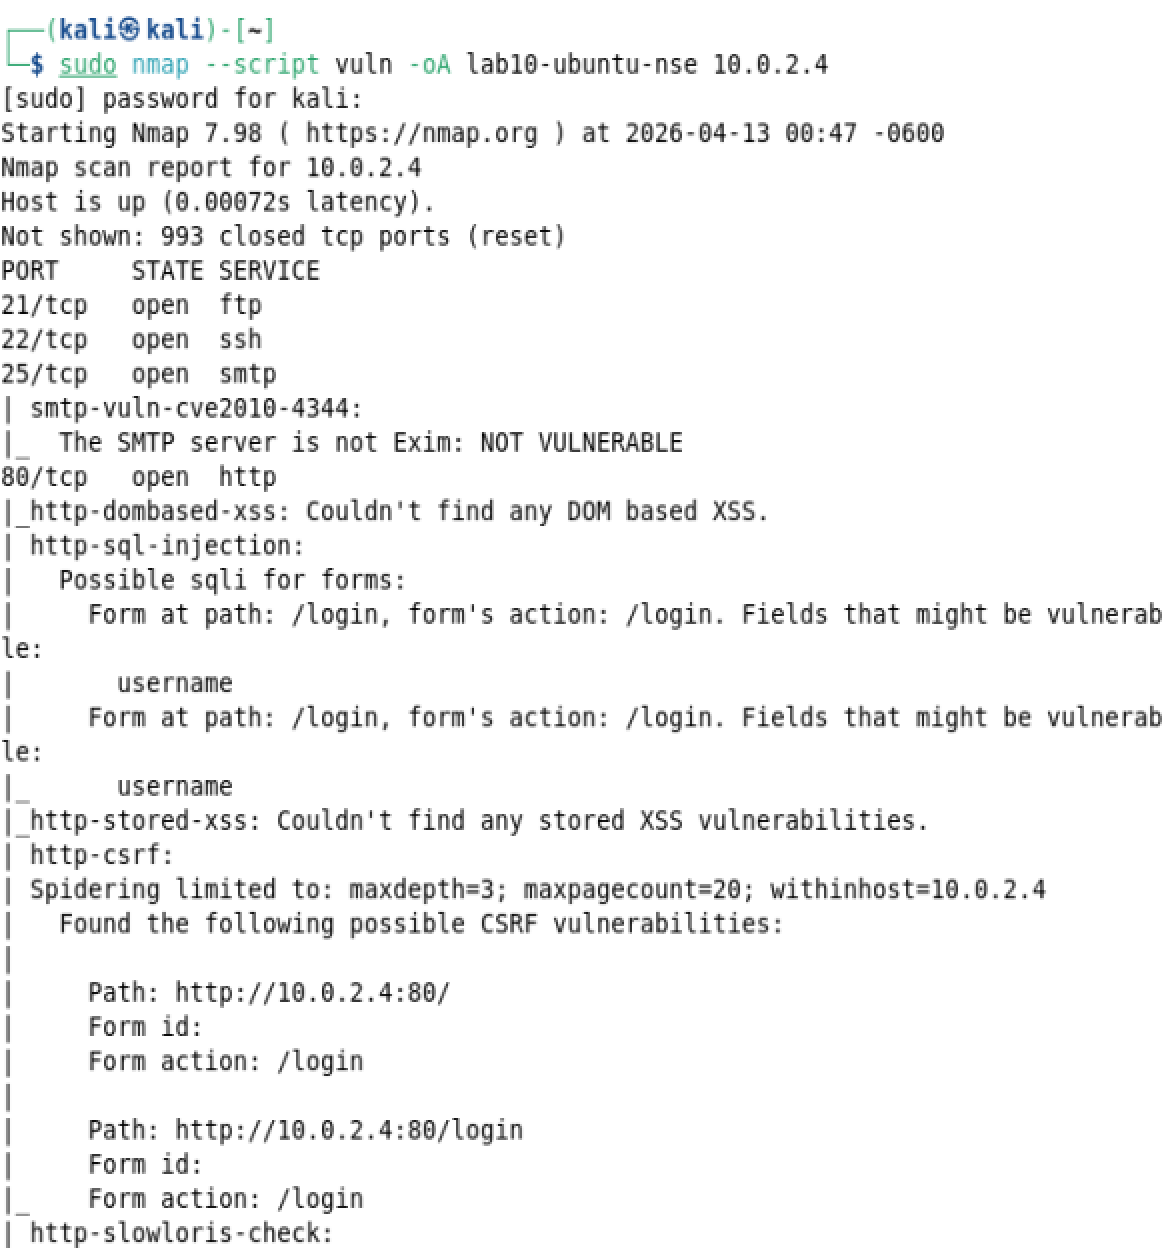
\includegraphics[width=0.50\textwidth]{images/2.1.1.png} 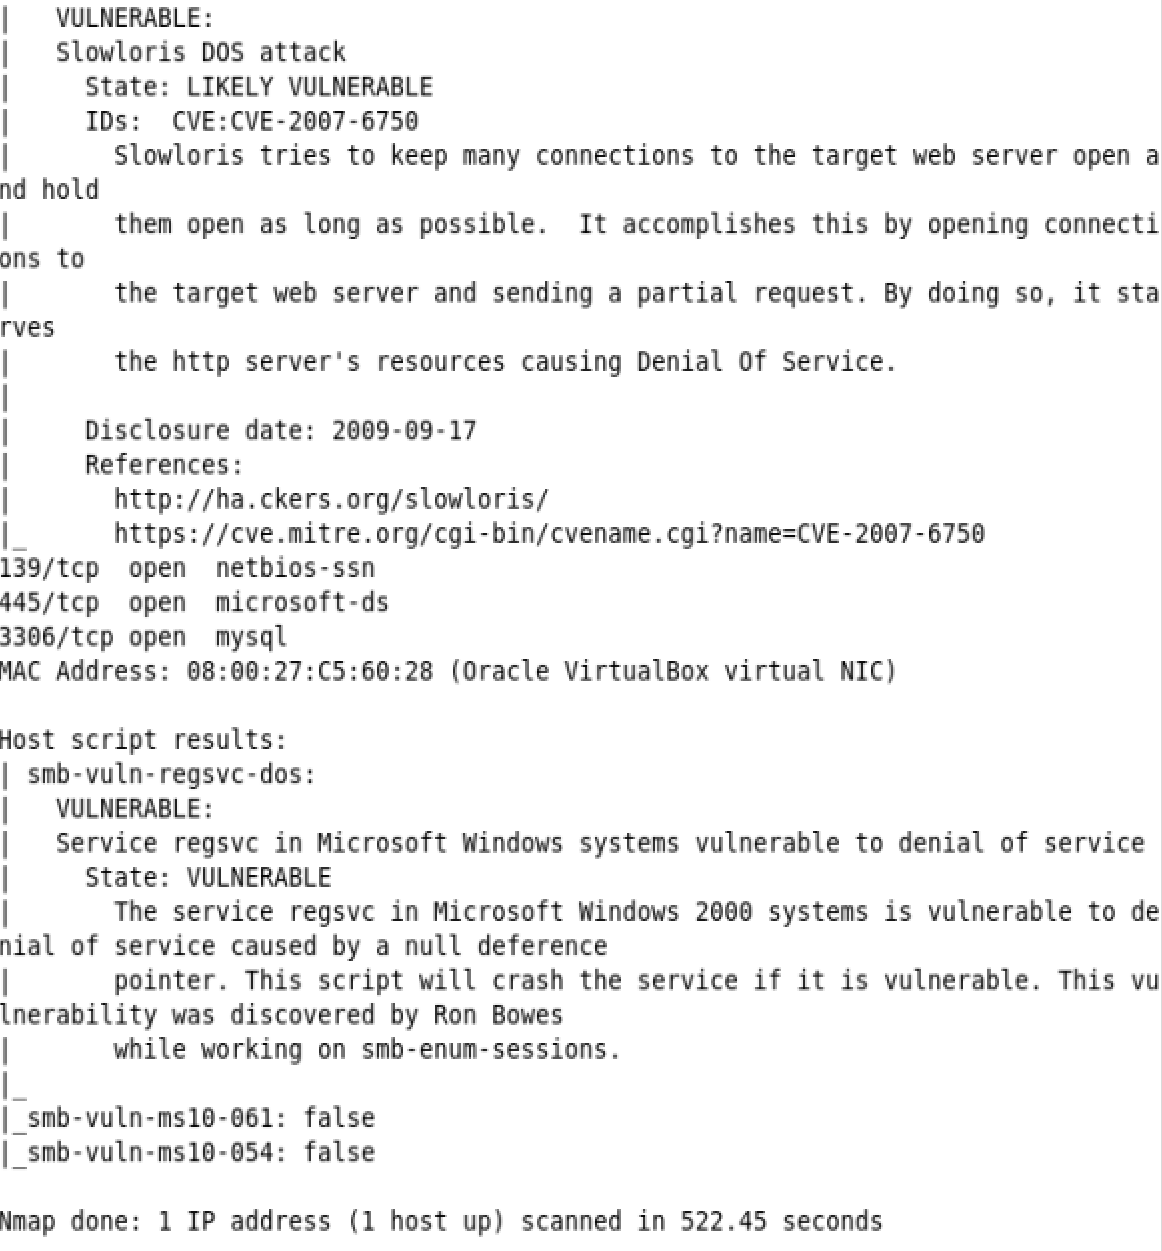
\includegraphics[width=0.50\textwidth]{images/2.1.2.png}\\ \textit{Figure 4: Nmap vulnerability scan results.}

% +++ 2.2 +++
\subsection{Targeted Service Scripts}
% +++ FTP (port 21) Scan +++
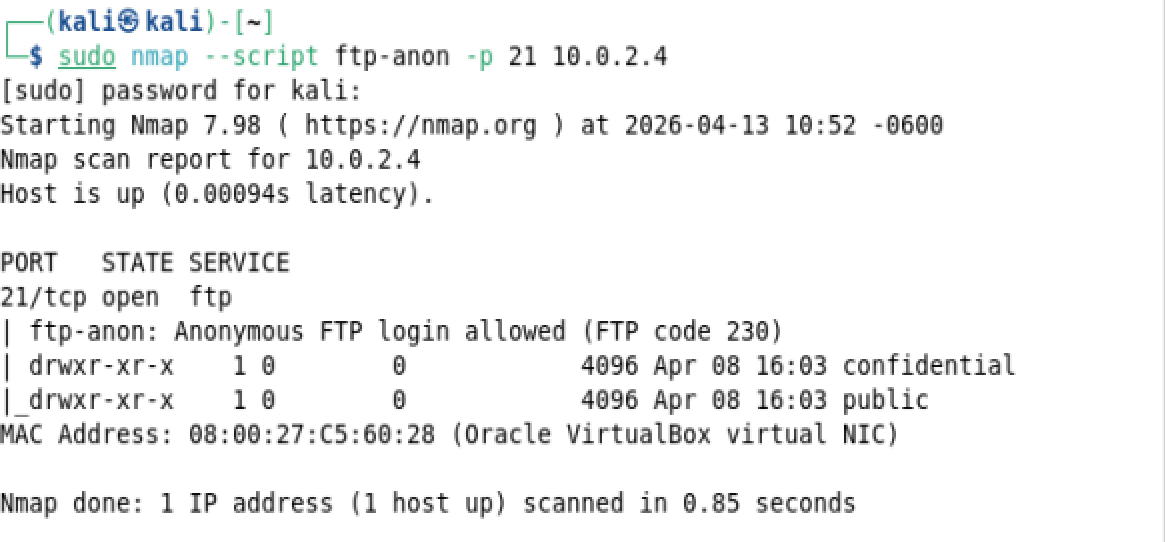
\includegraphics[width=0.50\textwidth]{images/2.2.1.png}\\ \textit{Figure 5: Nmap targeted FTP (port 21) service script results.}\\
% +++ SMB (port 445) Scan +++
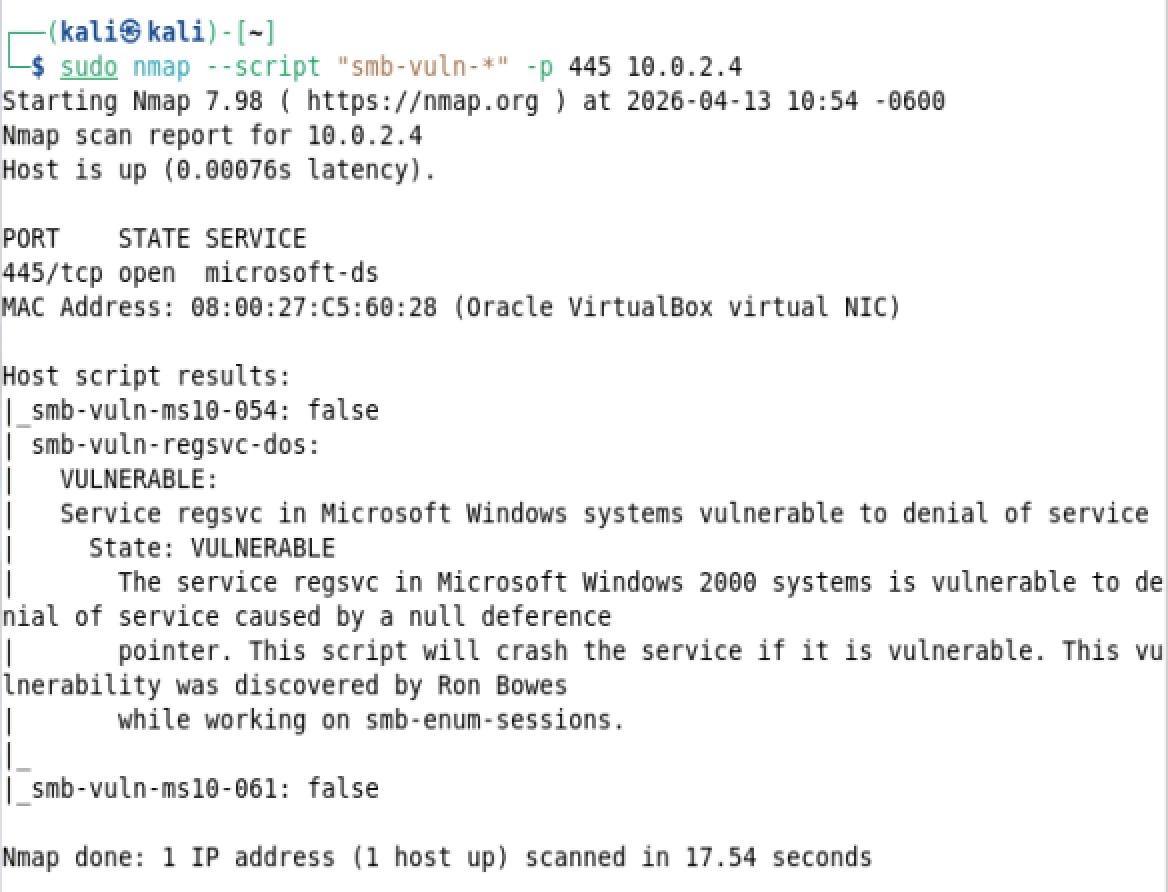
\includegraphics[width=0.50\textwidth]{images/2.2.2.png}\\ \textit{Figure 6: Nmap targeted SMB (port 445) service script results.}\\
\ \\
% +++ MySQL (port 3306) Scan +++
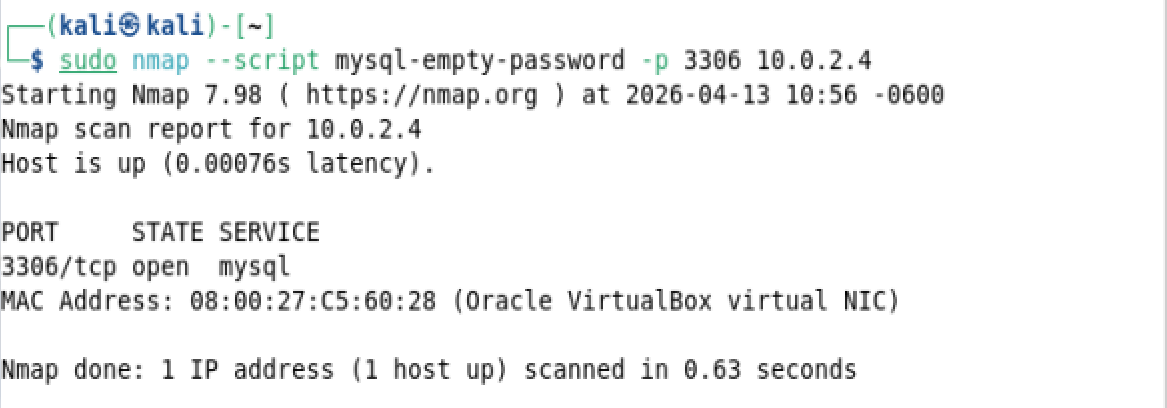
\includegraphics[width=0.50\textwidth]{images/2.2.3.png}\\ \textit{Figure 7: Nmap targeted MySQL (port 3306) service script results.}\\

% +++ 2.3 +++
\subsection{CVE Findings}
\textit{CVE-2002-0597 (Port 445)}
\begin{itemize}
	\item \textbf{CVSS Score:} 5.0 (Medium)
	\item \textbf{Description:} LANMAN service on Microsoft Windows 2000 allows remote attackers to cause a denial of service (CPU/memory exhaustion) via a stream of malformed data to microsoft-ds port 445.
\end{itemize}
\newpage
\textit{CVE-2026-33643 (Port 3306)}
\begin{itemize}
	\item \textbf{CVSS Score:} N/A (not yet scored)
	\item \textbf{Description:} SQL Injection vulnerability in SchemaHero 0.23.0 via the column parameter to the mysqlColumnAsInsert function in file plugins/mysql/lib/column.go.
\end{itemize}

% ++++ Part 03 ++++
\section{OpenVAS Full Scan}

% +++ 3.2 +++
\subsection{Creating a Scan Target}
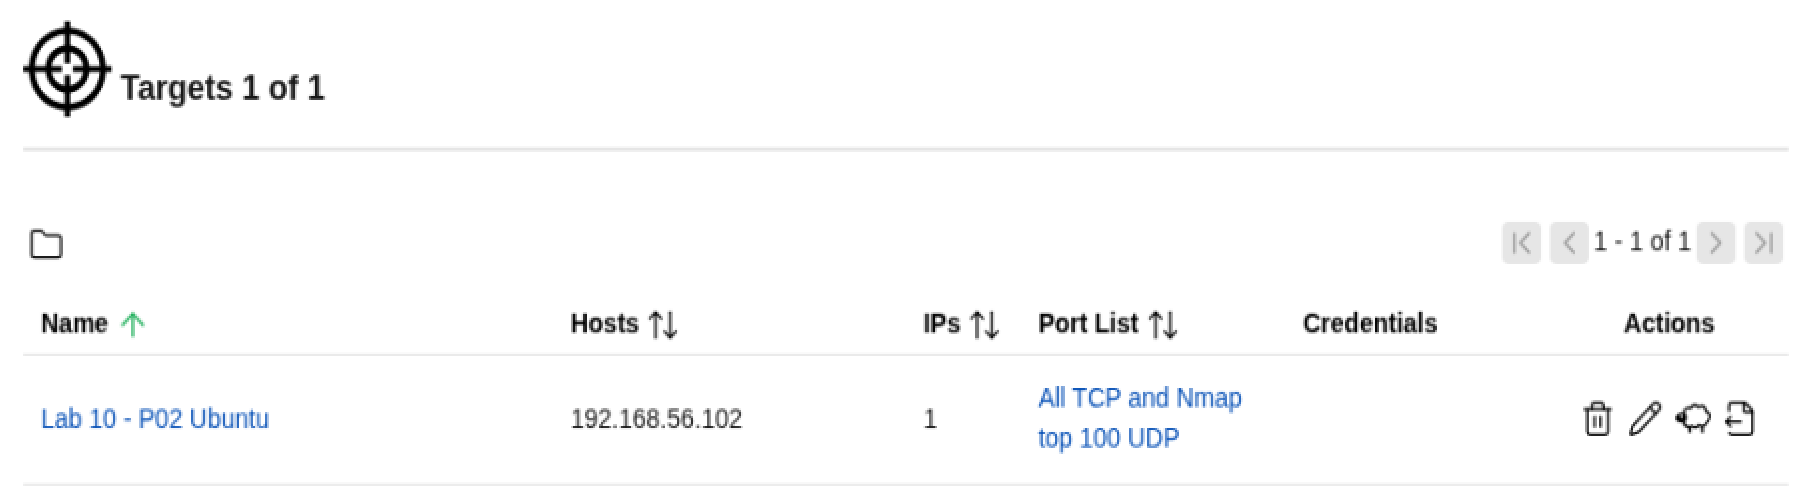
\includegraphics[width=0.50\textwidth]{images/3.1.png}\\ \textit{Figure 8: OpenVAS scan target configuration.}

% +++ 3.3 +++
\subsection{Creating and Running a Scan Task}
\textit{Note about the lab: This part was messy, to put it likely. I ran into one reoccurring problem over a couple of dozens of scans where the scans themselves just seemed to slide off of the target. Logs showed that ever scan was starting and ending without running any plugins against the target (although it was discovered alive). \\
After over six hours of troubleshooting, I nuked the gvm build and restarted from scratch. This still failed to fix the issue, so troubleshooting continued.\\
I started noticing that when I would check my ip addresses, one of the two channels on either of my machines would continually drop their IP and connection. With some help from Claude, I was able to force IP loads on both machines and I was able to download the needed plugins and run my scan.}
\newpage
\noindent 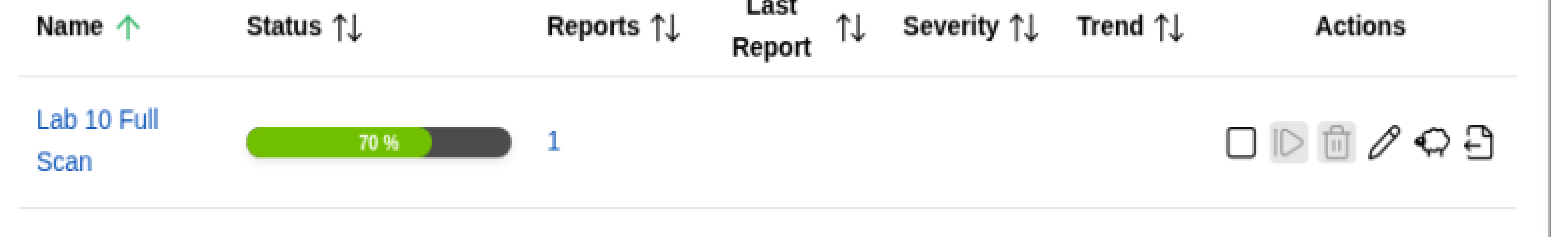
\includegraphics[width=0.50\textwidth]{images/3.2.png}\\ \textit{Figure 9: OpenVAS scan in progress.}\\
\ \\
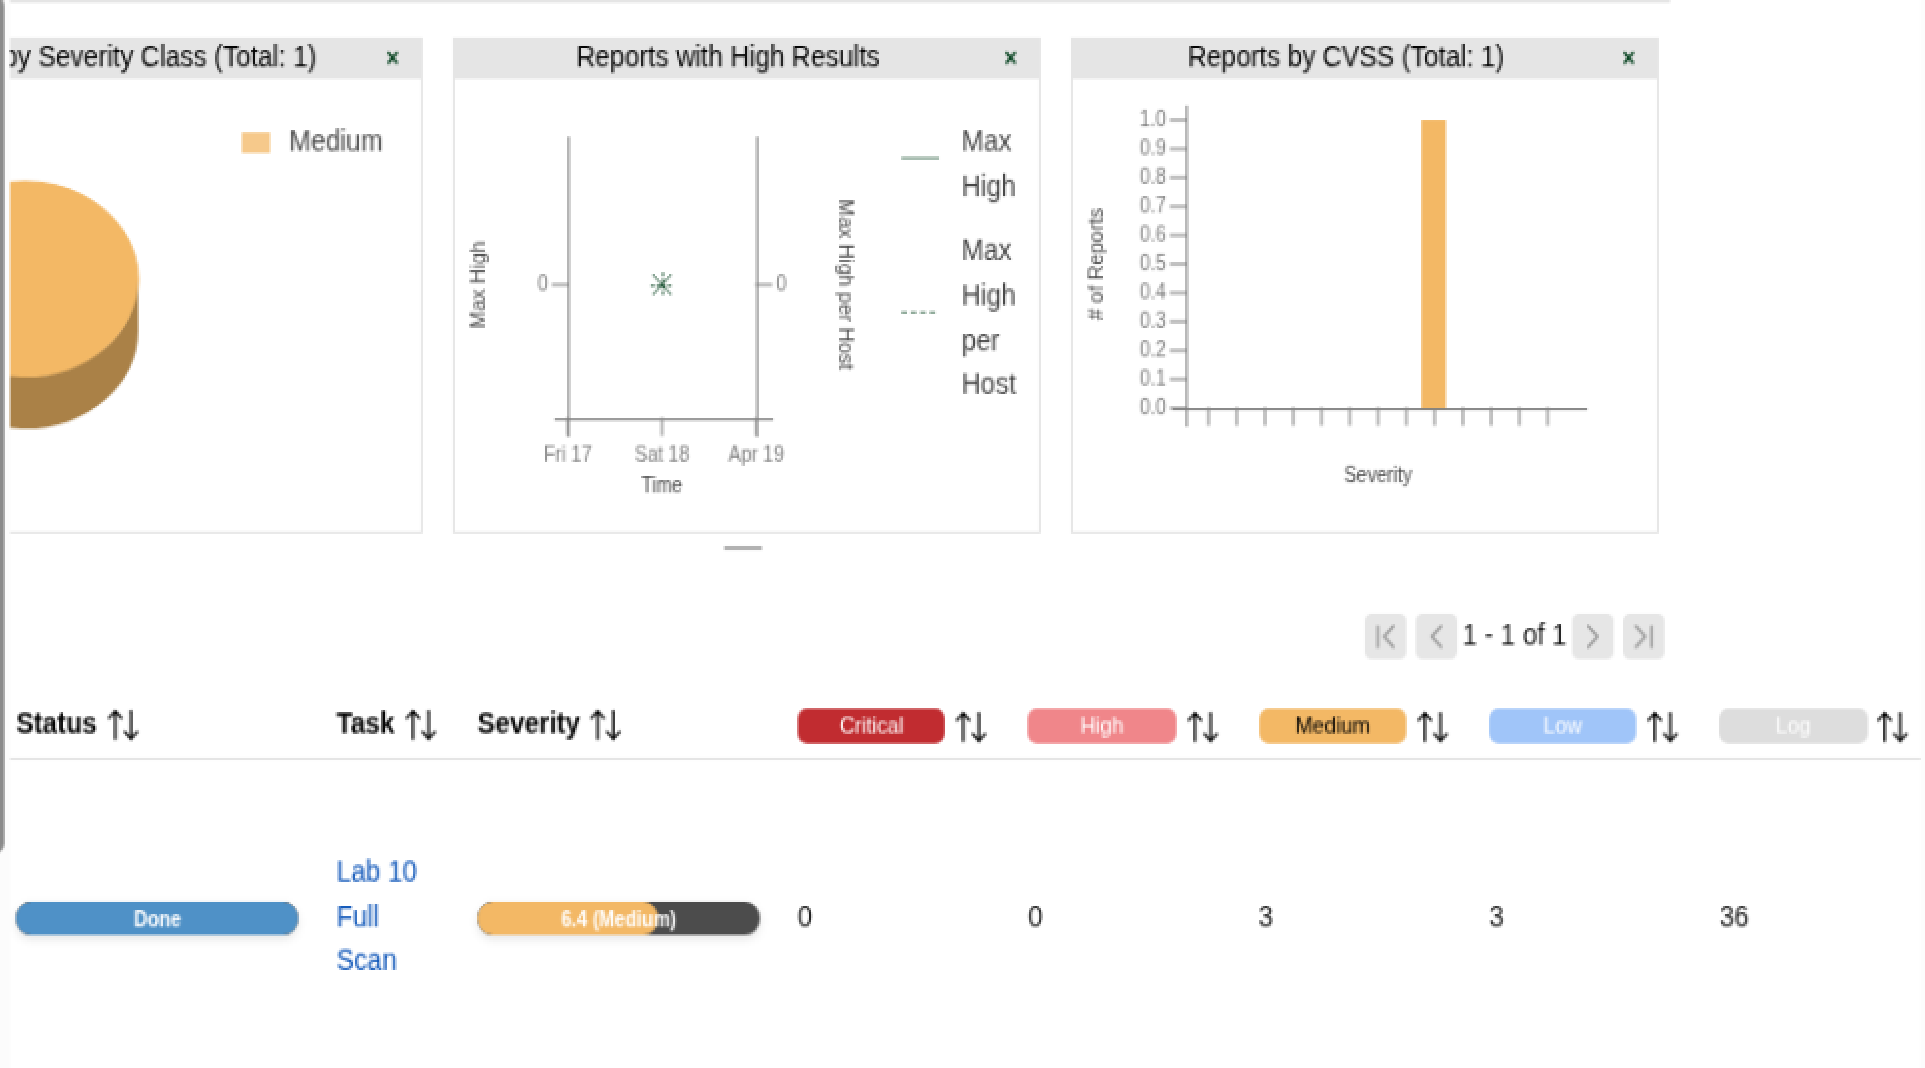
\includegraphics[width=0.50\textwidth]{images/3.3.1.png}\\ \textit{Figure 10: OpenVAS scan results.}\\
\ \\
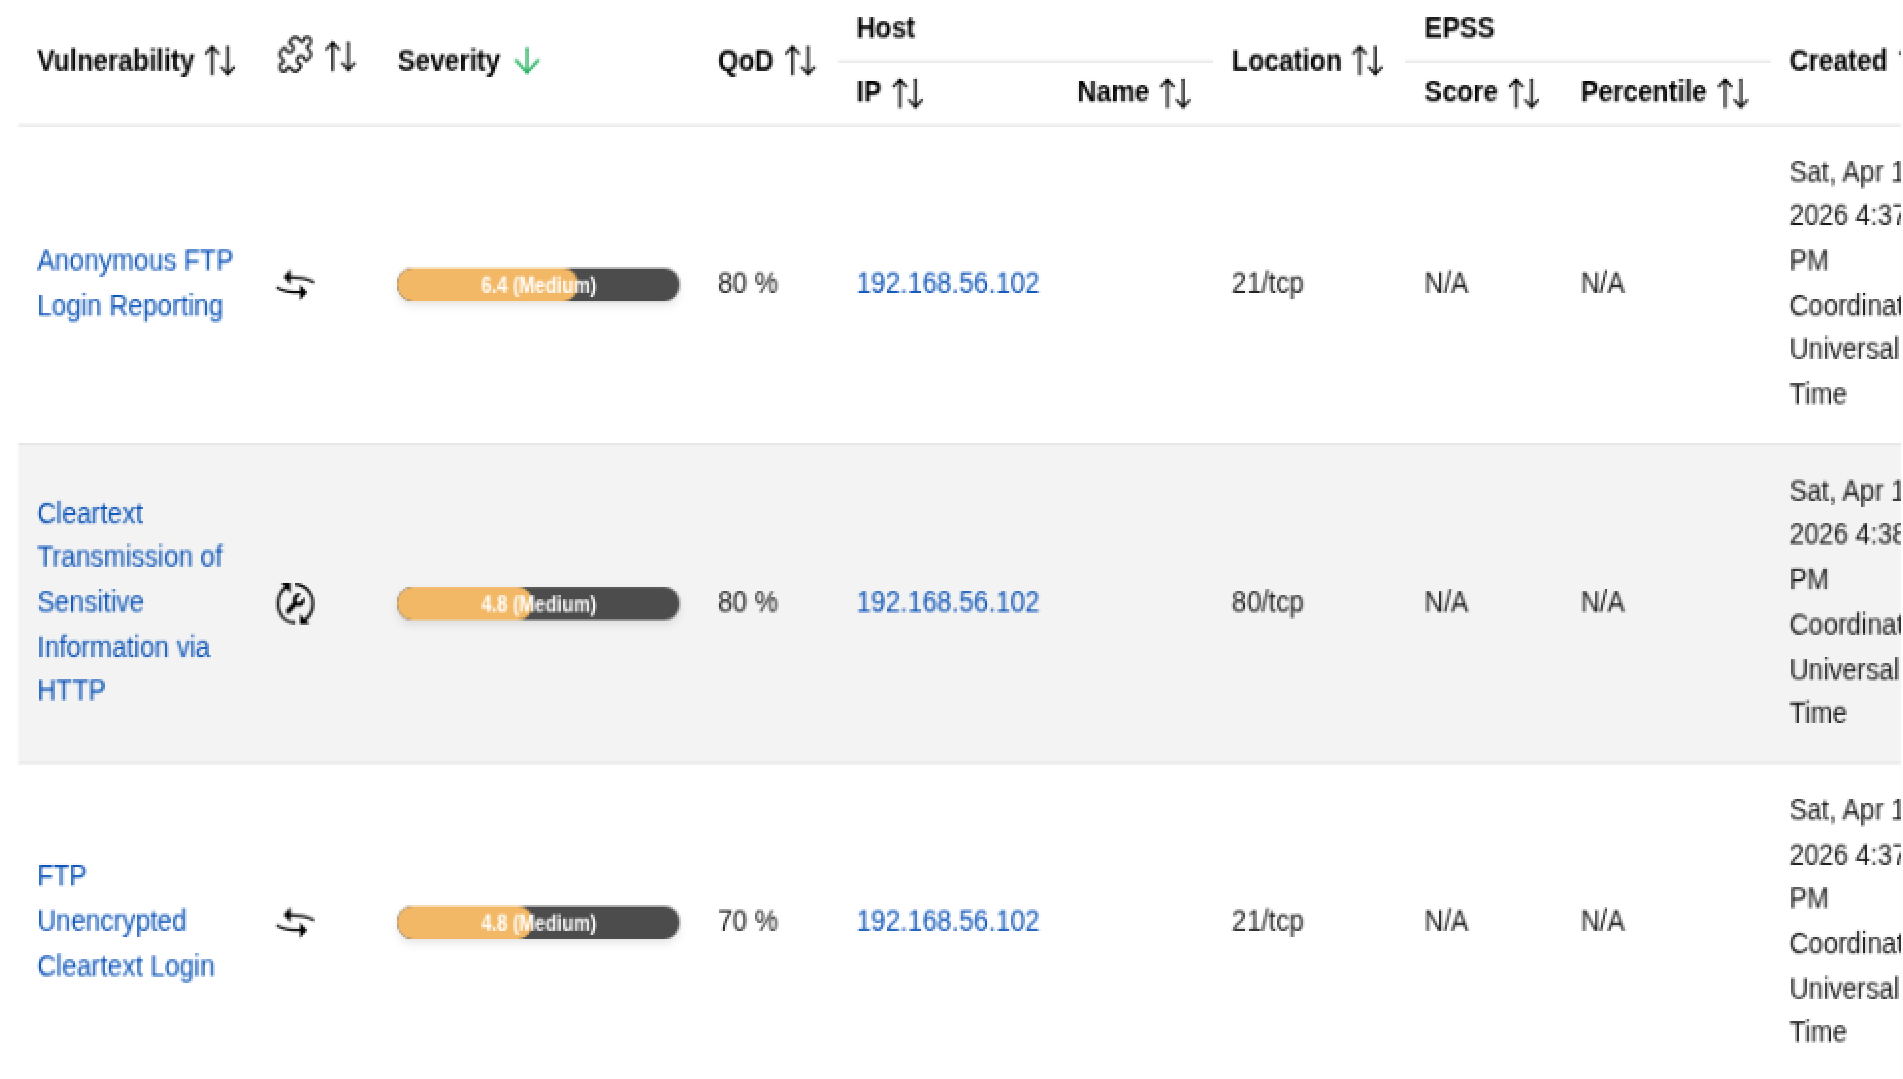
\includegraphics[width=0.45\textwidth]{images/3.3.2.png} 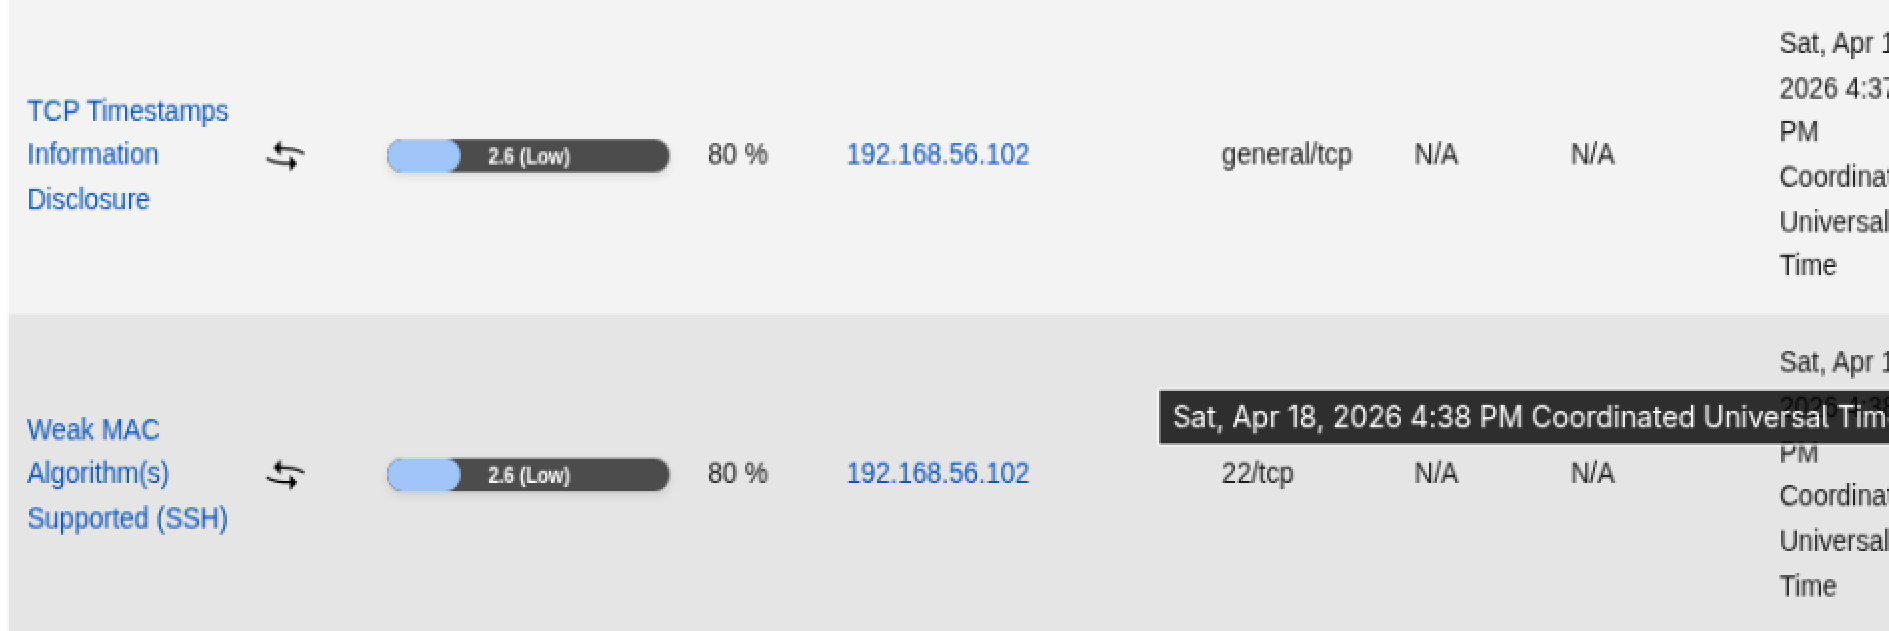
\includegraphics[width=0.45\textwidth]{images/3.3.3.png}\\ \textit{Figure 11: OpenVAS scan top 5 findings.}\\
\newpage

% ++++ Part 04 ++++
\section{Vulnerability Analysis \& Prioritization}

% +++ 4.1 +++
\subsection{Top-10 Findings}
\begin{longtable}{
    || >{\centering\arraybackslash}p{\colSmall}
    | >{\raggedright\arraybackslash}p{\colSmall}
    | >{\raggedright\arraybackslash}p{\colSmall}||}
    \hline\hline
    \multicolumn{3}{|c|}{\textbf{Priority}} \\
    \hline
    \cellcolor[HTML]{AE381B}\textbf{High} & \cellcolor[HTML]{E6A115}\textbf{Medium} & \cellcolor[HTML]{31728C}\textbf{Low} \\
    \hline\hline
\end{longtable}

{\singlespacing
	\begin{longtable}{
 		|| >{\centering\arraybackslash}p{\colNum}
  		| >{\raggedright\arraybackslash}p{\colSmall}
  		| >{\raggedright\arraybackslash}p{\colNum}
  		| >{\raggedright\arraybackslash}p{\colNum}
  		| >{\raggedright\arraybackslash}p{\colNum}
        | >{\raggedright\arraybackslash}p{\colNum}
  		| >{\raggedright\arraybackslash}p{\colSmall}
        | >{\raggedright\arraybackslash}p{\colSmall} ||}
		\hline
		\textbf{\#} & \small{\textbf{Finding}} & \small{\textbf{CVE}} & \footnotesize{\textbf{CVSS Score}} & \tiny{\textbf{Severity}} & \small{\textbf{Port}} & \small{\textbf{Description}} & \small{\textbf{Source}} \\
		\hline\hline
		\endhead
		\hline
 	    	 \cellcolor[HTML]{AE381B}1 & Anonymous FTP Login Reporting & CVE- 1999- 0497 & 6.4 & Med. & 21/ tcp & Reports if the remote FTP Server allows anonymous logins. & OpenVAS \\
		\hline
 	    	 \cellcolor[HTML]{E6A115}2 & DoS via LANMAN Service & CVE- 2002- 0597 & 5.0 & Med & 445/ tcp & Remote attackers can cause a denial of service via a stream of malformed data. & Nmap \\
		\hline
        	\cellcolor[HTML]{E6A115}3 & Cleartext Transmission of Sensitive Information via HTTP & N/A & 4.8 & Med. & 80/ tcp & Attacker could use this to compromise or eavesdrop on the HTTP comms between the client and server. & OpenVAS \\
		\hline
          	 \cellcolor[HTML]{AE381B}4 & Unencrypted Cleartext Login & N/A & 4.8  & Med. & 21/ tcp & The remote host is running an FTP service that allows cleartext logins over unencrypted connections. & OpenVAS \\
		\hline
     	   	\cellcolor[HTML]{E6A115}5 & SQL Injection via SchemaHero 0.23.0 & CVE- 2026- 33643 & N/A  & N/A & 3306/ tcp & SQL Injection vulnerability in SchemaHero 0.23.0 via the column parameter to the mysqlColumnAsInsert function in file plugins/mysql/lib/ column.go & Nmap \\
	    \hline
     		 \cellcolor[HTML]{31728C}6 & Weak MAC Algorithm Supported (SSH) & N/A & 2.6  & Low & 22/ tcp & The remote host supports a weak MAC algorithm in SSH connections. & OpenVAS \\
		\hline
     	   	 \cellcolor[HTML]{31728C}7 & TCP Timestamp Info Disclosure & N/A & 2.6  & Low & 22/ tcp & The remote host implements TCP timestamps and therefore allows to compute the uptime. & OpenVAS \\
		\hline
        	 \cellcolor[HTML]{31728C}8 & ICMP Timestamp Reply Information Disclosure & CVE- 1999- 0524 & 2.1  & Low & general/ icmp & The remote host resonded ton ICMP timestamp request. & OpenVAS\\
		\hline
	\end{longtable}
}
\noindent Note: First, I apologize for the short list. These were all the vulnerabilities that my scans were able to find.\\
Additionally, I want to note the process of making this list. The information contained comes directly from GreenBone/OpenVAS reports and nvd.nist.gov. However, when beginning my priority assessment, it was clear that some information would be difficult to obtain as every government site I accessed has a brief disclosure about funding cuts at the top. As such, I had a hard time finding information on CVEs older than a couple of years.\\
Since I hit this bump, I consulted with Claude to see what it thought of the list, what sort of information it could gather, and where it would get it from. It came up with sound reasoning behind its findings and let me know the following: \\
\textit{"One heads-up worth noting in your report: NVD is currently redirecting CVE detail pages rather than serving them directly, which is consistent with the funding/maintenance issues you mentioned. The scores I've cited come from Tenable, Greenbone/OpenVAS, and CVEdetails as secondary sources..."}

\subsection{Identifying False Positives}

Looking over my reports, only one of the findings stands out as a (most certain) false positive, that being \#2 on my lists: CVE-2002-0597. \\
The vulnerability according to NIST is described as: "LANMAN service on \textit{Microsoft Windows 2000} allows remote attackers to cause a denial of service (CPU/memory exhaustion) via a stream of malformed data to microsoft-ds port 445." \\
Admittedly, because I work with Windows machines regularly, I skimmed passed this as legitimate. After all, SQL injections are serious. But it kept bothering me until it finally clicked that the target is an Ubuntu machine, not Windows. \\
I think the status of this one as a false positive should be obvious as the vulnerability is just not compatible with the target's operating system.

\subsection{Making the Case}
Based on my findings and taking into consideration the tight window that Meridian Analytics has for immediate maintenance, I suggest that numbers 1, 4, and 3 from the list be fixed in the order given. This short-list contains three high-problem areas that should be addressed immediately as they make unwanted system access extremely easy. Fortunately, each of these fixes should be able to be implemented easily with little problem.

% ++++ Part 5 ++++
\section{Remediation Plan}

% +++ 5.1 +++
\subsection{Remediation Template}
\begin{itemize}
    \item \textbf{Vulnerability Name}: Anonymous FTP Login Reported
    \item \textbf{CVSS Score / Severity}: 6.4 / Medium
    \item \textbf{What Fixes It}: Disable anonymous logins by altering /etc/vsftpd.conf using the \texttt{sudo nano} command. 
        \begin{enumerate}
            \item Once open, find and alter the anonymous login line: \texttt{anonymous\underbar{   }enable=YES} to \texttt{NO} 
            \item If the line does not exist, add it to the file. 
            \item Restart the service with command \texttt{sudo systemctl restart vsftpd}.
        \end{enumerate}
    \item \textbf{Remediation Risk}: There will be a brief window of downtime when the service is restarted. All FTP transfers active at that moment will be dropped and may cause minor disruptions in production. Additionally, the \texttt{public} directory may suggest that there are dependencies using the anonymous FTP. Before running the fix, check this directory for dependencies and adjust accordingly.
    \item \textbf{Verification}: Run command \texttt{ftp 127.0.0.1} and attempt to log in anonymously. It should be rejected.
    \item \textbf{Priority}: Immediate
\end{itemize}
\newpage
\begin{itemize}
    \item \textbf{Vulnerability Name}: FTP Unencrypted Cleartext Login
    \item \textbf{CVSS Score / Severity}: 4.8 / Medium
    \item \textbf{What Fixes It}: Enable FTPS by following these steps:
        \begin{enumerate}
            \item Generate a self-signed SSL certificate by running command \texttt{sudo openssl req -x509 -nodes -days 365 -newkey rsa:2048 -keyout /etc/ssl/private/vsftpd.key -out /etc/ssl/certs/vsftpd.crt}. Fill out the fields when propted.
            \item Open the vsftpd config file with command \texttt{sudo nano /etc/vsftpd.conf}.
            \item Add/update the following lines:\\
                \texttt{ssl\underbar{   }enable=YES}\\
                \texttt{allow\underbar{   }anon\underbar{   }ssl=NO}\\
                \texttt{force\underbar{   }local\underbar{   }data\underbar{   }ssl=YES}\\
                \texttt{force\underbar{   }local\underbar{   }logins\underbar{   }ssl=YES}\\
                \texttt{ssl\underbar{   }tlsv1=YES}\\
                \texttt{ssl\underbar{   }sslv2=NO}\\
                \texttt{ssl\underbar{   }sslv3=NO}\\
                \texttt{rsa\underbar{   }cert\underbar{   }file=/etc/ssl/certs/vsftpd.crt}\\
                \texttt{rsa\underbar{   }private\underbar{   }key\underbar{   }file=/etc/ssl/private/vsftpd.key}
            \item Restart vsftpd by running command \texttt{sudo systemctl restart vsftpd}.    
        \end{enumerate}
    \item \textbf{Remediation Risk}: \textbf{Client compatibility breaks} - Any client that was connecting via plain FTP will stop working once \texttt{force\underbar{   }local\underbar{   }data\underbar{   }ssl=YES} and \texttt{force\underbar{   }local\underbar{   }logins\underbar{   }ssl=YES} are set. Because these lines are absolutely necessary for encryption, you must inventory all clients connecting to the server before implementing those lines.\\ \textbf{Firewall/Port Considerations} - FTPS can require additional ports beyond 21 to function. These ports will need to be defined in vsftpd.conf and opened in the firewall.\\ \textbf{Certificate management overhead} - Make note of when the certificate will expire as it will need to be renewed.\\ Consider a staged roll-out where FTPS is enabled alongside FTP and migrate clients before finalizing the change.
    \item \textbf{Verification}: Run command \texttt{curl --ssl-reqd ftp://127.0.0.1 -u username:password -k}. The -k flag ignores the self-signed cert warning. If it connects, the FTPS is working.
    \item \textbf{Priority}: Immediate
\end{itemize}
\hrule
\begin{itemize}
    \item \textbf{Vulnerability Name}: Cleartext Transmission of Sensitive Information via HTTP
    \item \textbf{CVSS Score / Severity}: 4.8 / Medium
    \item \textbf{What Fixes It}: This is a two part fix:
        \begin{itemize}
            \item \textbf{Part 1 - Enable HTTPS (SSL/TLS)}
                \begin{enumerate}
                    \item Create a certificate with the command \texttt{sudo openssl req -x509 -nodes -days 365 -newkey rsa:2048 -keyout /etc/ssl/private/medtech.key -out /etc/ssl/certs/medtech.crt}
                    \item Enable HTTPS in Werkzeug by running the following Python code:\\ 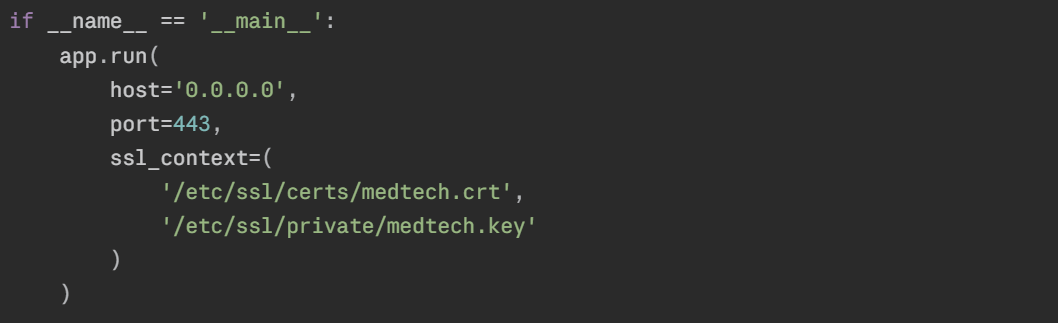
\includegraphics[width=0.50\textwidth]{images/5.1.1.png}
                \end{enumerate}
            \item \textbf{Part 2 - Force HTTP to HTTPS Redirect} by running the following Python code in Werkzeug:\\ 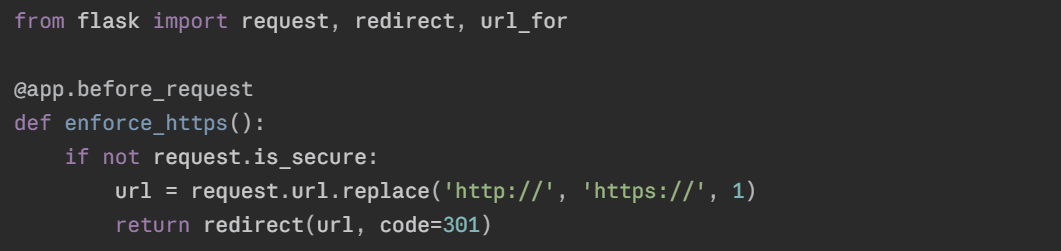
\includegraphics[width=0.50\textwidth]{images/5.1.2.png}
        \end{itemize}
    \item \textbf{Remediation Risk}: \textbf{Application Breakage} - If there are any hardcoded \texttt{http://} URLs internally, mixed content, or any interal service-to-service calls using plain HTTPS, they will break as soon as HTTPS is implemented. The entire codebase will have to be audited before and after the implementation. \textbf{Session and cookie invalidation} - Session cookies set without the \texttt{Secure} flag will not transfer to HTTPS. Existing user session will likely be lost. \textbf{Port conflicts} - Moving to port 443 means that it will need to be available and open. If there is anything else listening on port 443, it will create conflict. Additionally, port 80 will need to stay open for the redirect.
    \item \textbf{Verification}: Test the redirect by running command \texttt{curl -I https://192.168.56.102/login}. This should return \texttt{301 Moved Permanently}. Test the HTTPS connection by running command \texttt{curl -k https://192.168.56.102/login}. The -k flag bypasses the self-signed cert warning. If you get the login page back, HTTPS is working.
    \item \textbf{Priority}: Immediate
\end{itemize}

\vfill
\textit{++report written with (minimal) help from Claude (Sonnet 4.6)++}
\end{document}

% +++++++++ Helpful stuff +++++++++++
%
% +++ Using Minipages +++
% \begin{minipage}[t]{\linewidth}
% \includegraphics[width=0.50\textwidth]{*Image file}\\
% \textit{*Image subtitle}
% \end{minipage}
% \end{enumerate}
%

% +++ For tables that take multiple pages +++
%{\singlespacing
%	\begin{longtable}{
% 		|| >{\centering\arraybackslash}p{\colNum}
%  		| >{\raggedright\arraybackslash}p{\colSmall}
%  		| >{\raggedright\arraybackslash}p{\colSmall}
%  		| >{\raggedright\arraybackslash}p{\colBig}
%  		| >{\raggedright\arraybackslash}p{\colSmall} ||}
%		\hline
%		\textbf{x} & \textbf{x} & \textbf{x} & \textbf{x} & \textbf{x} \\
%		\hline\hline
%		\endhead
%		\hline
%  	    	 x & x & x & x  & x \\
%		\hline
%	\end{longtable}
%}












